\documentclass[twoside]{book}

% Packages required by doxygen
\usepackage{calc}
\usepackage{doxygen}
\usepackage{graphicx}
\usepackage[utf8]{inputenc}
\usepackage{makeidx}
\usepackage{multicol}
\usepackage{multirow}
\usepackage{textcomp}
\usepackage[table]{xcolor}

% Font selection
\usepackage[T1]{fontenc}
\usepackage{mathptmx}
\usepackage[scaled=.90]{helvet}
\usepackage{courier}
\usepackage{amssymb}
\usepackage{sectsty}
\renewcommand{\familydefault}{\sfdefault}
\allsectionsfont{%
  \fontseries{bc}\selectfont%
  \color{darkgray}%
}
\renewcommand{\DoxyLabelFont}{%
  \fontseries{bc}\selectfont%
  \color{darkgray}%
}

% Page & text layout
\usepackage{geometry}
\geometry{%
  a4paper,%
  top=2.5cm,%
  bottom=2.5cm,%
  left=2.5cm,%
  right=2.5cm%
}
\tolerance=750
\hfuzz=15pt
\hbadness=750
\setlength{\emergencystretch}{15pt}
\setlength{\parindent}{0cm}
\setlength{\parskip}{0.2cm}
\makeatletter
\renewcommand{\paragraph}{%
  \@startsection{paragraph}{4}{0ex}{-1.0ex}{1.0ex}{%
    \normalfont\normalsize\bfseries\SS@parafont%
  }%
}
\renewcommand{\subparagraph}{%
  \@startsection{subparagraph}{5}{0ex}{-1.0ex}{1.0ex}{%
    \normalfont\normalsize\bfseries\SS@subparafont%
  }%
}
\makeatother

% Headers & footers
\usepackage{fancyhdr}
\pagestyle{fancyplain}
\fancyhead[LE]{\fancyplain{}{\bfseries\thepage}}
\fancyhead[CE]{\fancyplain{}{}}
\fancyhead[RE]{\fancyplain{}{\bfseries\leftmark}}
\fancyhead[LO]{\fancyplain{}{\bfseries\rightmark}}
\fancyhead[CO]{\fancyplain{}{}}
\fancyhead[RO]{\fancyplain{}{\bfseries\thepage}}
\fancyfoot[LE]{\fancyplain{}{}}
\fancyfoot[CE]{\fancyplain{}{}}
\fancyfoot[RE]{\fancyplain{}{\bfseries\scriptsize Generated on Thu Feb 19 2015 11\-:37\-:52 for My Project by Doxygen }}
\fancyfoot[LO]{\fancyplain{}{\bfseries\scriptsize Generated on Thu Feb 19 2015 11\-:37\-:52 for My Project by Doxygen }}
\fancyfoot[CO]{\fancyplain{}{}}
\fancyfoot[RO]{\fancyplain{}{}}
\renewcommand{\footrulewidth}{0.4pt}
\renewcommand{\chaptermark}[1]{%
  \markboth{#1}{}%
}
\renewcommand{\sectionmark}[1]{%
  \markright{\thesection\ #1}%
}

% Indices & bibliography
\usepackage{natbib}
\usepackage[titles]{tocloft}
\setcounter{tocdepth}{3}
\setcounter{secnumdepth}{5}
\makeindex

% Hyperlinks (required, but should be loaded last)
\usepackage{ifpdf}
\ifpdf
  \usepackage[pdftex,pagebackref=true]{hyperref}
\else
  \usepackage[ps2pdf,pagebackref=true]{hyperref}
\fi
\hypersetup{%
  colorlinks=true,%
  linkcolor=blue,%
  citecolor=blue,%
  unicode%
}

% Custom commands
\newcommand{\clearemptydoublepage}{%
  \newpage{\pagestyle{empty}\cleardoublepage}%
}


%===== C O N T E N T S =====

\begin{document}

% Titlepage & ToC
\hypersetup{pageanchor=false}
\pagenumbering{roman}
\begin{titlepage}
\vspace*{7cm}
\begin{center}%
{\Large My Project }\\
\vspace*{1cm}
{\large Generated by Doxygen 1.8.6}\\
\vspace*{0.5cm}
{\small Thu Feb 19 2015 11:37:52}\\
\end{center}
\end{titlepage}
\clearemptydoublepage
\tableofcontents
\clearemptydoublepage
\pagenumbering{arabic}
\hypersetup{pageanchor=true}

%--- Begin generated contents ---
\chapter{Hierarchical Index}
\doxysection{Hierarquia de Classes}
Esta lista de hierarquias está parcialmente ordenada (ordem alfabética)\+:\begin{DoxyCompactList}
\item \contentsline{section}{CDiscretization}{\pageref{class_c_discretization}}{}
\item \contentsline{section}{CFluido}{\pageref{class_c_fluido}}{}
\begin{DoxyCompactList}
\item \contentsline{section}{CGas}{\pageref{class_c_gas}}{}
\item \contentsline{section}{CLiquido}{\pageref{class_c_liquido}}{}
\end{DoxyCompactList}
\item \contentsline{section}{CGnuplot}{\pageref{class_c_gnuplot}}{}
\item \contentsline{section}{CGrid}{\pageref{class_c_grid}}{}
\item \contentsline{section}{CMatrix}{\pageref{class_c_matrix}}{}
\item \contentsline{section}{CProps}{\pageref{class_c_props}}{}
\item \contentsline{section}{CReservoir}{\pageref{class_c_reservoir}}{}
\item \contentsline{section}{CSimulador\+Monofasico2D}{\pageref{class_c_simulador_monofasico2_d}}{}
\item \contentsline{section}{CWell}{\pageref{class_c_well}}{}
\end{DoxyCompactList}

\chapter{Class Index}
\doxysection{Lista de Classes}
Aqui estão as classes, estruturas, uniões e interfaces e suas respectivas descrições\+:\begin{DoxyCompactList}
\item\contentsline{section}{\mbox{\hyperlink{class_c_discretization}{CDiscretization}} }{\pageref{class_c_discretization}}{}
\item\contentsline{section}{\mbox{\hyperlink{class_c_fluido}{CFluido}} }{\pageref{class_c_fluido}}{}
\item\contentsline{section}{\mbox{\hyperlink{class_c_gas}{CGas}} }{\pageref{class_c_gas}}{}
\item\contentsline{section}{\mbox{\hyperlink{class_c_gnuplot}{CGnuplot}} }{\pageref{class_c_gnuplot}}{}
\item\contentsline{section}{\mbox{\hyperlink{class_c_grid}{CGrid}} }{\pageref{class_c_grid}}{}
\item\contentsline{section}{\mbox{\hyperlink{class_c_liquido}{CLiquido}} }{\pageref{class_c_liquido}}{}
\item\contentsline{section}{\mbox{\hyperlink{class_c_props}{CProps}} }{\pageref{class_c_props}}{}
\item\contentsline{section}{\mbox{\hyperlink{class_c_reservoir}{CReservoir}} }{\pageref{class_c_reservoir}}{}
\item\contentsline{section}{\mbox{\hyperlink{class_c_simulador}{CSimulador}} }{\pageref{class_c_simulador}}{}
\item\contentsline{section}{\mbox{\hyperlink{class_c_well}{CWell}} }{\pageref{class_c_well}}{}
\end{DoxyCompactList}

\chapter{Class Documentation}
\hypertarget{classCAplicacao}{\section{C\-Aplicacao Class Reference}
\label{classCAplicacao}\index{C\-Aplicacao@{C\-Aplicacao}}
}


{\ttfamily \#include $<$C\-Aplicacao.\-h$>$}

\subsection*{Public Member Functions}
\begin{DoxyCompactItemize}
\item 
void \hyperlink{classCAplicacao_a47bf6fb7afc11f9966a52ccfdb13673e}{Run} ()
\begin{DoxyCompactList}\small\item\em Método de execução da aplicação. \end{DoxyCompactList}\end{DoxyCompactItemize}


\subsection{Detailed Description}
Declara uma classe minimalista, a classe \hyperlink{classCAplicacao}{C\-Aplicacao} A mesma inclui apenas um método, o método \hyperlink{classCAplicacao_a47bf6fb7afc11f9966a52ccfdb13673e}{Run()}. 

\subsection{Member Function Documentation}
\hypertarget{classCAplicacao_a47bf6fb7afc11f9966a52ccfdb13673e}{\index{C\-Aplicacao@{C\-Aplicacao}!Run@{Run}}
\index{Run@{Run}!CAplicacao@{C\-Aplicacao}}
\subsubsection[{Run}]{\setlength{\rightskip}{0pt plus 5cm}void C\-Aplicacao\-::\-Run (
\begin{DoxyParamCaption}
{}
\end{DoxyParamCaption}
)}}\label{classCAplicacao_a47bf6fb7afc11f9966a52ccfdb13673e}


Método de execução da aplicação. 

Inclui a declaração da classe.

Este programa exemplifica a estrutura/layout de um programa típico em C++\-Implementa os métodos da classe O método \hyperlink{classCAplicacao_a47bf6fb7afc11f9966a52ccfdb13673e}{Run()} escreve uma mensagem na tela 

The documentation for this class was generated from the following files\-:\begin{DoxyCompactItemize}
\item 
C\-Aplicacao.\-h\item 
C\-Aplicacao.\-cpp\end{DoxyCompactItemize}

\hypertarget{classGnuplot}{\section{Gnuplot Class Reference}
\label{classGnuplot}\index{Gnuplot@{Gnuplot}}
}


Classe de interface para acesso ao programa gnuplot.  




{\ttfamily \#include $<$cgnuplot.\-h$>$}

\subsection*{Public Member Functions}
\begin{DoxyCompactItemize}
\item 
\hypertarget{classGnuplot_a187eb517b362cf379492fe7f1621ee50}{\hyperlink{classGnuplot_a187eb517b362cf379492fe7f1621ee50}{Gnuplot} (const std\-::string \&style=\char`\"{}points\char`\"{})}\label{classGnuplot_a187eb517b362cf379492fe7f1621ee50}

\begin{DoxyCompactList}\small\item\em Construtor, seta o estilo do grafico na construcao. \end{DoxyCompactList}\item 
\hypertarget{classGnuplot_a8ceac5808e42665c1dee305ae7ea9070}{\hyperlink{classGnuplot_a8ceac5808e42665c1dee305ae7ea9070}{Gnuplot} (const std\-::vector$<$ double $>$ \&x, const std\-::string \&title=\char`\"{}\char`\"{}, const std\-::string \&style=\char`\"{}points\char`\"{}, const std\-::string \&labelx=\char`\"{}x\char`\"{}, const std\-::string \&labely=\char`\"{}y\char`\"{})}\label{classGnuplot_a8ceac5808e42665c1dee305ae7ea9070}

\begin{DoxyCompactList}\small\item\em Construtor, plota um grafico a partir dde um vector, diretamente na construcao. \end{DoxyCompactList}\item 
\hypertarget{classGnuplot_a24327b6116c71acdc195eadf665c67cb}{\hyperlink{classGnuplot_a24327b6116c71acdc195eadf665c67cb}{Gnuplot} (const std\-::vector$<$ double $>$ \&x, const std\-::vector$<$ double $>$ \&y, const std\-::string \&title=\char`\"{}\char`\"{}, const std\-::string \&style=\char`\"{}points\char`\"{}, const std\-::string \&labelx=\char`\"{}x\char`\"{}, const std\-::string \&labely=\char`\"{}y\char`\"{})}\label{classGnuplot_a24327b6116c71acdc195eadf665c67cb}

\begin{DoxyCompactList}\small\item\em Construtor, plota um grafico do tipo x\-\_\-y a partir de vetores, diretamente na construcao. \end{DoxyCompactList}\item 
\hypertarget{classGnuplot_a14191e89154f2716608f6907975cc012}{\hyperlink{classGnuplot_a14191e89154f2716608f6907975cc012}{Gnuplot} (const std\-::vector$<$ double $>$ \&x, const std\-::vector$<$ double $>$ \&y, const std\-::vector$<$ double $>$ \&z, const std\-::string \&title=\char`\"{}\char`\"{}, const std\-::string \&style=\char`\"{}points\char`\"{}, const std\-::string \&labelx=\char`\"{}x\char`\"{}, const std\-::string \&labely=\char`\"{}y\char`\"{}, const std\-::string \&labelz=\char`\"{}z\char`\"{})}\label{classGnuplot_a14191e89154f2716608f6907975cc012}

\begin{DoxyCompactList}\small\item\em Construtor, plota um grafico de x\-\_\-y\-\_\-z a partir de vetores, diretamente na construcao. \end{DoxyCompactList}\item 
\hypertarget{classGnuplot_a78a68f621caa87d1f34324fcd093c7bd}{\hyperlink{classGnuplot_a78a68f621caa87d1f34324fcd093c7bd}{$\sim$\-Gnuplot} ()}\label{classGnuplot_a78a68f621caa87d1f34324fcd093c7bd}

\begin{DoxyCompactList}\small\item\em Destrutor, necessario para deletar arquivos temporarios. \end{DoxyCompactList}\item 
\hypertarget{classGnuplot_a07607803ede8dd5416906df0a1924fc5}{\hyperlink{classGnuplot}{Gnuplot} \& \hyperlink{classGnuplot_a07607803ede8dd5416906df0a1924fc5}{cmd} (const std\-::string \&cmdstr)}\label{classGnuplot_a07607803ede8dd5416906df0a1924fc5}

\begin{DoxyCompactList}\small\item\em Envia comando para o gnuplot. \end{DoxyCompactList}\item 
\hypertarget{classGnuplot_af9ffb5b4c18cdf7c56e5c446f72e515d}{\hyperlink{classGnuplot}{Gnuplot} \& \hyperlink{classGnuplot_af9ffb5b4c18cdf7c56e5c446f72e515d}{Cmd} (const std\-::string \&cmdstr)}\label{classGnuplot_af9ffb5b4c18cdf7c56e5c446f72e515d}

\begin{DoxyCompactList}\small\item\em Envia comando para o gnuplot. \end{DoxyCompactList}\item 
\hypertarget{classGnuplot_a0d6db1521e789d7b73415ce85b723046}{\hyperlink{classGnuplot}{Gnuplot} \& \hyperlink{classGnuplot_a0d6db1521e789d7b73415ce85b723046}{Command} (const std\-::string \&cmdstr)}\label{classGnuplot_a0d6db1521e789d7b73415ce85b723046}

\begin{DoxyCompactList}\small\item\em Envia comando para o gnuplot. \end{DoxyCompactList}\item 
\hypertarget{classGnuplot_ae56495dc15f23d32f099129d3a50dd6c}{\hyperlink{classGnuplot}{Gnuplot} \& \hyperlink{classGnuplot_ae56495dc15f23d32f099129d3a50dd6c}{operator$<$$<$} (const std\-::string \&cmdstr)}\label{classGnuplot_ae56495dc15f23d32f099129d3a50dd6c}

\begin{DoxyCompactList}\small\item\em Sobrecarga operador $<$$<$, funciona como Comando. \end{DoxyCompactList}\item 
\hypertarget{classGnuplot_a356d2faaa79f08d13fec9718b776b28d}{\hyperlink{classGnuplot}{Gnuplot} \& \hyperlink{classGnuplot_a356d2faaa79f08d13fec9718b776b28d}{showonscreen} ()}\label{classGnuplot_a356d2faaa79f08d13fec9718b776b28d}

\begin{DoxyCompactList}\small\item\em Mostrar na tela ou escrever no arquivo, seta o tipo de terminal para terminal\-\_\-std. \end{DoxyCompactList}\item 
\hypertarget{classGnuplot_aee70cb6dfc893d6f19976fa9042c8e7c}{\hyperlink{classGnuplot}{Gnuplot} \& \hyperlink{classGnuplot_aee70cb6dfc893d6f19976fa9042c8e7c}{Show\-On\-Screen} ()}\label{classGnuplot_aee70cb6dfc893d6f19976fa9042c8e7c}

\begin{DoxyCompactList}\small\item\em Mostrar na tela ou escrever no arquivo, seta o tipo de terminal para terminal\-\_\-std. \end{DoxyCompactList}\item 
\hypertarget{classGnuplot_a032072c7c01b508a7535a17fb08562b1}{\hyperlink{classGnuplot}{Gnuplot} \& \hyperlink{classGnuplot_a032072c7c01b508a7535a17fb08562b1}{savetops} (const std\-::string \&filename=\char`\"{}gnuplot\-\_\-output\char`\"{})}\label{classGnuplot_a032072c7c01b508a7535a17fb08562b1}

\begin{DoxyCompactList}\small\item\em Salva sessao do gnuplot para um arquivo postscript, nome do arquivo sem extensao. \end{DoxyCompactList}\item 
\hypertarget{classGnuplot_a5adf74dfda6d9d70a16c435fedf07625}{\hyperlink{classGnuplot}{Gnuplot} \& \hyperlink{classGnuplot_a5adf74dfda6d9d70a16c435fedf07625}{Save\-Tops} (const std\-::string \&filename=\char`\"{}gnuplot\-\_\-output\char`\"{})}\label{classGnuplot_a5adf74dfda6d9d70a16c435fedf07625}

\begin{DoxyCompactList}\small\item\em Salva sessao do gnuplot para um arquivo postscript, nome do arquivo sem extensao. \end{DoxyCompactList}\item 
\hypertarget{classGnuplot_acfdcda292650775ebed4683e8e1515b5}{\hyperlink{classGnuplot}{Gnuplot} \& \hyperlink{classGnuplot_acfdcda292650775ebed4683e8e1515b5}{set\-\_\-style} (const std\-::string \&stylestr=\char`\"{}points\char`\"{})}\label{classGnuplot_acfdcda292650775ebed4683e8e1515b5}

\begin{DoxyCompactList}\small\item\em Seta estilos de linhas (em alguns casos sao necessarias informacoes adicionais). lines, points, linespoints, impulses, dots, steps, fsteps, histeps, boxes, histograms, filledcurves. \end{DoxyCompactList}\item 
\hypertarget{classGnuplot_ae64e911770994ba05cc2f6dcbfe31540}{\hyperlink{classGnuplot}{Gnuplot} \& \hyperlink{classGnuplot_ae64e911770994ba05cc2f6dcbfe31540}{Style} (const std\-::string \&stylestr=\char`\"{}points\char`\"{})}\label{classGnuplot_ae64e911770994ba05cc2f6dcbfe31540}

\begin{DoxyCompactList}\small\item\em Seta estilos de linhas (em alguns casos sao necessarias informacoes adicionais). lines, points, linespoints, impulses, dots, steps, fsteps, histeps, boxes, histograms, filledcurves. \end{DoxyCompactList}\item 
\hypertarget{classGnuplot_aa18386919da2ec4c994f1f9c7195d384}{\hyperlink{classGnuplot}{Gnuplot} \& \hyperlink{classGnuplot_aa18386919da2ec4c994f1f9c7195d384}{set\-\_\-smooth} (const std\-::string \&stylestr=\char`\"{}csplines\char`\"{})}\label{classGnuplot_aa18386919da2ec4c994f1f9c7195d384}

\begin{DoxyCompactList}\small\item\em Ativa suavizacao. Argumentos para interpolacoes e aproximacoes. csplines, bezier, acsplines (para dados com valor $>$ 0), sbezier, unique, frequency (funciona somente com plot\-\_\-x, plot\-\_\-xy, plotfile\-\_\-x, plotfile\-\_\-xy (se a suavizacao esta ativa, set\-\_\-style nao tem efeito na plotagem dos graficos) \end{DoxyCompactList}\item 
\hypertarget{classGnuplot_aec18795f217d6d8791275a1c866b550e}{\hyperlink{classGnuplot}{Gnuplot} \& \hyperlink{classGnuplot_aec18795f217d6d8791275a1c866b550e}{unset\-\_\-smooth} ()}\label{classGnuplot_aec18795f217d6d8791275a1c866b550e}

\begin{DoxyCompactList}\small\item\em Desativa suavizacao. \end{DoxyCompactList}\item 
\hypertarget{classGnuplot_aedd7a473c34c83b3b9ec1cea9891d0f2}{\hyperlink{classGnuplot}{Gnuplot} \& \hyperlink{classGnuplot_aedd7a473c34c83b3b9ec1cea9891d0f2}{Smooth} (const std\-::string \&stylestr=\char`\"{}csplines\char`\"{})}\label{classGnuplot_aedd7a473c34c83b3b9ec1cea9891d0f2}

\begin{DoxyCompactList}\small\item\em Ativa suavizacao. Argumentos para interpolacoes e aproximacoes. csplines, bezier, acsplines (para dados com valor $>$ 0), sbezier, unique, frequency (funciona somente com plot\-\_\-x, plot\-\_\-xy, plotfile\-\_\-x, plotfile\-\_\-xy (se a suavizacao esta ativa, set\-\_\-style nao tem efeito na plotagem dos graficos) \end{DoxyCompactList}\item 
\hypertarget{classGnuplot_a9eaf8050edfad9d926d41b102d2f24cb}{\hyperlink{classGnuplot}{Gnuplot} \& {\bfseries Smooth} (int \-\_\-fsmooth)}\label{classGnuplot_a9eaf8050edfad9d926d41b102d2f24cb}

\item 
\hyperlink{classGnuplot}{Gnuplot} \& \hyperlink{classGnuplot_a95ec1636a871447dfe99463b769339c7}{set\-\_\-pointsize} (const double pointsize=1.\-0)
\begin{DoxyCompactList}\small\item\em Desativa suavizacao. \end{DoxyCompactList}\item 
\hypertarget{classGnuplot_adb4a794cf81d9b615f133feca1e917e8}{\hyperlink{classGnuplot}{Gnuplot} \& \hyperlink{classGnuplot_adb4a794cf81d9b615f133feca1e917e8}{Point\-Size} (const double pointsize=1.\-0)}\label{classGnuplot_adb4a794cf81d9b615f133feca1e917e8}

\begin{DoxyCompactList}\small\item\em Escala o tamanho do ponto usado na plotagem. \end{DoxyCompactList}\item 
\hypertarget{classGnuplot_a4b7245b12dad1c0ef326e5f59eb83001}{\hyperlink{classGnuplot}{Gnuplot} \& \hyperlink{classGnuplot_a4b7245b12dad1c0ef326e5f59eb83001}{set\-\_\-grid} ()}\label{classGnuplot_a4b7245b12dad1c0ef326e5f59eb83001}

\begin{DoxyCompactList}\small\item\em Ativa o grid (padrao = desativado). \end{DoxyCompactList}\item 
\hypertarget{classGnuplot_a8b9a16d5793c3f4939b917b2c263860c}{\hyperlink{classGnuplot}{Gnuplot} \& \hyperlink{classGnuplot_a8b9a16d5793c3f4939b917b2c263860c}{unset\-\_\-grid} ()}\label{classGnuplot_a8b9a16d5793c3f4939b917b2c263860c}

\begin{DoxyCompactList}\small\item\em Desativa o grid (padrao = desativado). \end{DoxyCompactList}\item 
\hypertarget{classGnuplot_a67e669cdac3b09ae16678f5211dda786}{\hyperlink{classGnuplot}{Gnuplot} \& \hyperlink{classGnuplot_a67e669cdac3b09ae16678f5211dda786}{Grid} (bool \-\_\-fgrid=1)}\label{classGnuplot_a67e669cdac3b09ae16678f5211dda786}

\begin{DoxyCompactList}\small\item\em Ativa/\-Desativa o grid (padrao = desativado). \end{DoxyCompactList}\item 
\hypertarget{classGnuplot_a671cbe7b18a267ea59f532c83a0035f6}{\hyperlink{classGnuplot}{Gnuplot} \& \hyperlink{classGnuplot_a671cbe7b18a267ea59f532c83a0035f6}{set\-\_\-samples} (const int samples=100)}\label{classGnuplot_a671cbe7b18a267ea59f532c83a0035f6}

\begin{DoxyCompactList}\small\item\em Seta taxa de amostragem das funcoes, ou dos dados de interpolacao. \end{DoxyCompactList}\item 
\hypertarget{classGnuplot_a0be7d1bfb41fd1e44969361ab02320b9}{\hyperlink{classGnuplot}{Gnuplot} \& \hyperlink{classGnuplot_a0be7d1bfb41fd1e44969361ab02320b9}{Samples} (const int samples=100)}\label{classGnuplot_a0be7d1bfb41fd1e44969361ab02320b9}

\begin{DoxyCompactList}\small\item\em Seta taxa de amostragem das funcoes, ou dos dados de interpolacao. \end{DoxyCompactList}\item 
\hypertarget{classGnuplot_ab810fa4c02fb49ae197786c305b78702}{\hyperlink{classGnuplot}{Gnuplot} \& \hyperlink{classGnuplot_ab810fa4c02fb49ae197786c305b78702}{set\-\_\-isosamples} (const int isolines=10)}\label{classGnuplot_ab810fa4c02fb49ae197786c305b78702}

\begin{DoxyCompactList}\small\item\em Seta densidade de isolinhas para plotagem de funcoes como superficies (para plotagen 3d). \end{DoxyCompactList}\item 
\hypertarget{classGnuplot_a215f314f3bcc2c869e7379a9728e5f95}{\hyperlink{classGnuplot}{Gnuplot} \& \hyperlink{classGnuplot_a215f314f3bcc2c869e7379a9728e5f95}{Iso\-Samples} (const int isolines=10)}\label{classGnuplot_a215f314f3bcc2c869e7379a9728e5f95}

\begin{DoxyCompactList}\small\item\em Seta densidade de isolinhas para plotagem de funcoes como superficies (para plotagen 3d). \end{DoxyCompactList}\item 
\hypertarget{classGnuplot_a5ada5c76db0a735d3d331caa0eb4968a}{\hyperlink{classGnuplot}{Gnuplot} \& \hyperlink{classGnuplot_a5ada5c76db0a735d3d331caa0eb4968a}{set\-\_\-hidden3d} ()}\label{classGnuplot_a5ada5c76db0a735d3d331caa0eb4968a}

\begin{DoxyCompactList}\small\item\em Ativa remocao de linhas ocultas na plotagem de superficies (para plotagen 3d). \end{DoxyCompactList}\item 
\hypertarget{classGnuplot_a763ff17df1679cc2b1463b024aa89ebc}{\hyperlink{classGnuplot}{Gnuplot} \& \hyperlink{classGnuplot_a763ff17df1679cc2b1463b024aa89ebc}{unset\-\_\-hidden3d} ()}\label{classGnuplot_a763ff17df1679cc2b1463b024aa89ebc}

\begin{DoxyCompactList}\small\item\em Desativa remocao de linhas ocultas na plotagem de superficies (para plotagen 3d). \end{DoxyCompactList}\item 
\hypertarget{classGnuplot_a9004d7b6d322be1eeb32eb8eb0c25487}{\hyperlink{classGnuplot}{Gnuplot} \& \hyperlink{classGnuplot_a9004d7b6d322be1eeb32eb8eb0c25487}{Hidden3d} (bool \-\_\-fhidden3d=1)}\label{classGnuplot_a9004d7b6d322be1eeb32eb8eb0c25487}

\begin{DoxyCompactList}\small\item\em Ativa/\-Desativa remocao de linhas ocultas na plotagem de superficies (para plotagen 3d). \end{DoxyCompactList}\item 
\hyperlink{classGnuplot}{Gnuplot} \& \hyperlink{classGnuplot_af845efc728a90d7e10de764eff0b2423}{set\-\_\-contour} (const std\-::string \&position=\char`\"{}base\char`\"{})
\begin{DoxyCompactList}\small\item\em Ativa desenho do contorno em superficies (para plotagen 3d). \end{DoxyCompactList}\item 
\hypertarget{classGnuplot_a39d10e6ce85875939a9c594d132a10d7}{\hyperlink{classGnuplot}{Gnuplot} \& \hyperlink{classGnuplot_a39d10e6ce85875939a9c594d132a10d7}{unset\-\_\-contour} ()}\label{classGnuplot_a39d10e6ce85875939a9c594d132a10d7}

\begin{DoxyCompactList}\small\item\em Desativa desenho do contorno em superficies (para plotagen 3d). \end{DoxyCompactList}\item 
\hyperlink{classGnuplot}{Gnuplot} \& \hyperlink{classGnuplot_a826a0f860cd984748f8c7ee80228fce7}{Contour} (const std\-::string \&position=\char`\"{}base\char`\"{})
\begin{DoxyCompactList}\small\item\em Ativa/\-Desativa desenho do contorno em superficies (para plotagen 3d). \end{DoxyCompactList}\item 
\hypertarget{classGnuplot_ab2918e5653c9d421bf924d7dc2467429}{\hyperlink{classGnuplot}{Gnuplot} \& {\bfseries Contour} (int \-\_\-fcontour)}\label{classGnuplot_ab2918e5653c9d421bf924d7dc2467429}

\item 
\hypertarget{classGnuplot_a0e36dcd81618234c6cdd135a9e1eee2b}{\hyperlink{classGnuplot}{Gnuplot} \& \hyperlink{classGnuplot_a0e36dcd81618234c6cdd135a9e1eee2b}{set\-\_\-surface} ()}\label{classGnuplot_a0e36dcd81618234c6cdd135a9e1eee2b}

\begin{DoxyCompactList}\small\item\em Ativa a visualizacao da superficie (para plotagen 3d). \end{DoxyCompactList}\item 
\hypertarget{classGnuplot_a805f1807c9b3a0a6745d66fa1729e3be}{\hyperlink{classGnuplot}{Gnuplot} \& \hyperlink{classGnuplot_a805f1807c9b3a0a6745d66fa1729e3be}{unset\-\_\-surface} ()}\label{classGnuplot_a805f1807c9b3a0a6745d66fa1729e3be}

\begin{DoxyCompactList}\small\item\em Desativa a visualizacao da superficie (para plotagen 3d). \end{DoxyCompactList}\item 
\hypertarget{classGnuplot_a7b338ff4ec6c49659cd2022b68c0e861}{\hyperlink{classGnuplot}{Gnuplot} \& \hyperlink{classGnuplot_a7b338ff4ec6c49659cd2022b68c0e861}{Surface} (int \-\_\-fsurface=1)}\label{classGnuplot_a7b338ff4ec6c49659cd2022b68c0e861}

\begin{DoxyCompactList}\small\item\em Ativa/\-Desativa a visualizacao da superficie (para plotagen 3d). \end{DoxyCompactList}\item 
\hypertarget{classGnuplot_ad64a717dac18167f656c4f09239973f8}{\hyperlink{classGnuplot}{Gnuplot} \& \hyperlink{classGnuplot_ad64a717dac18167f656c4f09239973f8}{set\-\_\-legend} (const std\-::string \&position=\char`\"{}default\char`\"{})}\label{classGnuplot_ad64a717dac18167f656c4f09239973f8}

\begin{DoxyCompactList}\small\item\em Ativa a legenda (a legenda é setada por padrao). Posicao\-: inside/outside, left/center/right, top/center/bottom, nobox/box. \end{DoxyCompactList}\item 
\hypertarget{classGnuplot_a584e0710d7f5bcaa35653d1987f1563e}{\hyperlink{classGnuplot}{Gnuplot} \& \hyperlink{classGnuplot_a584e0710d7f5bcaa35653d1987f1563e}{unset\-\_\-legend} ()}\label{classGnuplot_a584e0710d7f5bcaa35653d1987f1563e}

\begin{DoxyCompactList}\small\item\em Desativa a legenda (a legenda é setada por padrao). \end{DoxyCompactList}\item 
\hypertarget{classGnuplot_aec3037a558d26535e3847c52d1b120aa}{\hyperlink{classGnuplot}{Gnuplot} \& \hyperlink{classGnuplot_aec3037a558d26535e3847c52d1b120aa}{Legend} (const std\-::string \&position=\char`\"{}default\char`\"{})}\label{classGnuplot_aec3037a558d26535e3847c52d1b120aa}

\begin{DoxyCompactList}\small\item\em Ativa/\-Desativa a legenda (a legenda é setada por padrao). \end{DoxyCompactList}\item 
\hypertarget{classGnuplot_a781ffec9b2ddd9706823b865acb95d0b}{\hyperlink{classGnuplot}{Gnuplot} \& \hyperlink{classGnuplot_a781ffec9b2ddd9706823b865acb95d0b}{Legend} (int \-\_\-flegend)}\label{classGnuplot_a781ffec9b2ddd9706823b865acb95d0b}

\begin{DoxyCompactList}\small\item\em Ativa/\-Desativa a legenda (a legenda é setada por padrao). \end{DoxyCompactList}\item 
\hypertarget{classGnuplot_aa693e806a115af1e2776a15078e75b46}{\hyperlink{classGnuplot}{Gnuplot} \& \hyperlink{classGnuplot_aa693e806a115af1e2776a15078e75b46}{set\-\_\-title} (const std\-::string \&title=\char`\"{}\char`\"{})}\label{classGnuplot_aa693e806a115af1e2776a15078e75b46}

\begin{DoxyCompactList}\small\item\em Ativa o titulo da secao do gnuplot. \end{DoxyCompactList}\item 
\hypertarget{classGnuplot_a0d205a55ae104403292622b49af14ae7}{\hyperlink{classGnuplot}{Gnuplot} \& \hyperlink{classGnuplot_a0d205a55ae104403292622b49af14ae7}{unset\-\_\-title} ()}\label{classGnuplot_a0d205a55ae104403292622b49af14ae7}

\begin{DoxyCompactList}\small\item\em Desativa o titulo da secao do gnuplot. \end{DoxyCompactList}\item 
\hypertarget{classGnuplot_a73bb8c97a946cafea0eca683450a6a62}{\hyperlink{classGnuplot}{Gnuplot} \& \hyperlink{classGnuplot_a73bb8c97a946cafea0eca683450a6a62}{Title} (const std\-::string \&title=\char`\"{}\char`\"{})}\label{classGnuplot_a73bb8c97a946cafea0eca683450a6a62}

\begin{DoxyCompactList}\small\item\em Ativa/\-Desativa o titulo da secao do gnuplot. \end{DoxyCompactList}\item 
\hypertarget{classGnuplot_afeab18e210616ae239adb7d816ecb2e9}{\hyperlink{classGnuplot}{Gnuplot} \& {\bfseries Title} (int \-\_\-ftitle)}\label{classGnuplot_afeab18e210616ae239adb7d816ecb2e9}

\item 
\hypertarget{classGnuplot_a7654b86e3873aec4c5101abb466fe4ab}{\hyperlink{classGnuplot}{Gnuplot} \& \hyperlink{classGnuplot_a7654b86e3873aec4c5101abb466fe4ab}{set\-\_\-ylabel} (const std\-::string \&label=\char`\"{}y\char`\"{})}\label{classGnuplot_a7654b86e3873aec4c5101abb466fe4ab}

\begin{DoxyCompactList}\small\item\em Seta o rotulo (nome) do eixo y. \end{DoxyCompactList}\item 
\hypertarget{classGnuplot_ab4cdb8c1abd919b9851ca9a81667f2a4}{\hyperlink{classGnuplot}{Gnuplot} \& \hyperlink{classGnuplot_ab4cdb8c1abd919b9851ca9a81667f2a4}{Y\-Label} (const std\-::string \&label=\char`\"{}y\char`\"{})}\label{classGnuplot_ab4cdb8c1abd919b9851ca9a81667f2a4}

\begin{DoxyCompactList}\small\item\em Seta o rotulo (nome) do eixo y. \end{DoxyCompactList}\item 
\hypertarget{classGnuplot_a58808028aec03a22b5c19693b14baeef}{\hyperlink{classGnuplot}{Gnuplot} \& \hyperlink{classGnuplot_a58808028aec03a22b5c19693b14baeef}{set\-\_\-xlabel} (const std\-::string \&label=\char`\"{}x\char`\"{})}\label{classGnuplot_a58808028aec03a22b5c19693b14baeef}

\begin{DoxyCompactList}\small\item\em Seta o rotulo (nome) do eixo x. \end{DoxyCompactList}\item 
\hypertarget{classGnuplot_ac36ea75f0759c98da946389e60c12278}{\hyperlink{classGnuplot}{Gnuplot} \& \hyperlink{classGnuplot_ac36ea75f0759c98da946389e60c12278}{X\-Label} (const std\-::string \&label=\char`\"{}x\char`\"{})}\label{classGnuplot_ac36ea75f0759c98da946389e60c12278}

\begin{DoxyCompactList}\small\item\em Seta o rotulo (nome) do eixo x. \end{DoxyCompactList}\item 
\hypertarget{classGnuplot_ab3206e715d20f05cc0dd1eec89ce8b07}{\hyperlink{classGnuplot}{Gnuplot} \& \hyperlink{classGnuplot_ab3206e715d20f05cc0dd1eec89ce8b07}{set\-\_\-zlabel} (const std\-::string \&label=\char`\"{}z\char`\"{})}\label{classGnuplot_ab3206e715d20f05cc0dd1eec89ce8b07}

\begin{DoxyCompactList}\small\item\em Seta o rotulo (nome) do eixo z. \end{DoxyCompactList}\item 
\hypertarget{classGnuplot_ace776aa2b273c0ec934e856cb28416eb}{\hyperlink{classGnuplot}{Gnuplot} \& \hyperlink{classGnuplot_ace776aa2b273c0ec934e856cb28416eb}{Z\-Label} (const std\-::string \&label=\char`\"{}z\char`\"{})}\label{classGnuplot_ace776aa2b273c0ec934e856cb28416eb}

\begin{DoxyCompactList}\small\item\em Seta o rotulo (nome) do eixo z. \end{DoxyCompactList}\item 
\hypertarget{classGnuplot_a726232ac7226b9fc8811eaefa87c902b}{\hyperlink{classGnuplot}{Gnuplot} \& \hyperlink{classGnuplot_a726232ac7226b9fc8811eaefa87c902b}{set\-\_\-xrange} (const int i\-From, const int i\-To)}\label{classGnuplot_a726232ac7226b9fc8811eaefa87c902b}

\begin{DoxyCompactList}\small\item\em Seta intervalo do eixo x. \end{DoxyCompactList}\item 
\hypertarget{classGnuplot_a3fb5c7726e954739d847edd2670705fe}{\hyperlink{classGnuplot}{Gnuplot} \& \hyperlink{classGnuplot_a3fb5c7726e954739d847edd2670705fe}{X\-Range} (const int i\-From, const int i\-To)}\label{classGnuplot_a3fb5c7726e954739d847edd2670705fe}

\begin{DoxyCompactList}\small\item\em Seta intervalo do eixo x. \end{DoxyCompactList}\item 
\hypertarget{classGnuplot_af621a43664a07523f098ffc3fb5a99b0}{\hyperlink{classGnuplot}{Gnuplot} \& \hyperlink{classGnuplot_af621a43664a07523f098ffc3fb5a99b0}{set\-\_\-yrange} (const int i\-From, const int i\-To)}\label{classGnuplot_af621a43664a07523f098ffc3fb5a99b0}

\begin{DoxyCompactList}\small\item\em Seta intervalo do eixo y. \end{DoxyCompactList}\item 
\hypertarget{classGnuplot_a266411505d17e3f85ceebd252b9e5fe9}{\hyperlink{classGnuplot}{Gnuplot} \& \hyperlink{classGnuplot_a266411505d17e3f85ceebd252b9e5fe9}{Y\-Range} (const int i\-From, const int i\-To)}\label{classGnuplot_a266411505d17e3f85ceebd252b9e5fe9}

\begin{DoxyCompactList}\small\item\em Seta intervalo do eixo y. \end{DoxyCompactList}\item 
\hypertarget{classGnuplot_a91666451b8cfd1c5b279d2e585b11af6}{\hyperlink{classGnuplot}{Gnuplot} \& \hyperlink{classGnuplot_a91666451b8cfd1c5b279d2e585b11af6}{set\-\_\-zrange} (const int i\-From, const int i\-To)}\label{classGnuplot_a91666451b8cfd1c5b279d2e585b11af6}

\begin{DoxyCompactList}\small\item\em Seta intervalo do eixo z. \end{DoxyCompactList}\item 
\hypertarget{classGnuplot_a8331c7ee5d65be5f4d88922a0b2f5d35}{\hyperlink{classGnuplot}{Gnuplot} \& \hyperlink{classGnuplot_a8331c7ee5d65be5f4d88922a0b2f5d35}{Z\-Range} (const int i\-From, const int i\-To)}\label{classGnuplot_a8331c7ee5d65be5f4d88922a0b2f5d35}

\begin{DoxyCompactList}\small\item\em Seta intervalo do eixo z. \end{DoxyCompactList}\item 
\hypertarget{classGnuplot_a453688dc2eb979f842082290f3c02ac3}{\hyperlink{classGnuplot}{Gnuplot} \& \hyperlink{classGnuplot_a453688dc2eb979f842082290f3c02ac3}{set\-\_\-xautoscale} ()}\label{classGnuplot_a453688dc2eb979f842082290f3c02ac3}

\begin{DoxyCompactList}\small\item\em Seta escalonamento automatico do eixo x (default). \end{DoxyCompactList}\item 
\hypertarget{classGnuplot_a4260baaa8fa1c269dd6eec31dcada605}{\hyperlink{classGnuplot}{Gnuplot} \& \hyperlink{classGnuplot_a4260baaa8fa1c269dd6eec31dcada605}{X\-Autoscale} ()}\label{classGnuplot_a4260baaa8fa1c269dd6eec31dcada605}

\begin{DoxyCompactList}\small\item\em Seta escalonamento automatico do eixo x (default). \end{DoxyCompactList}\item 
\hypertarget{classGnuplot_a3cc19dba32bb2d3ac59494ae1493faa7}{\hyperlink{classGnuplot}{Gnuplot} \& \hyperlink{classGnuplot_a3cc19dba32bb2d3ac59494ae1493faa7}{set\-\_\-yautoscale} ()}\label{classGnuplot_a3cc19dba32bb2d3ac59494ae1493faa7}

\begin{DoxyCompactList}\small\item\em Seta escalonamento automatico do eixo y (default). \end{DoxyCompactList}\item 
\hypertarget{classGnuplot_a288c0be86e20ff6986f5b43cb69b2bb0}{\hyperlink{classGnuplot}{Gnuplot} \& \hyperlink{classGnuplot_a288c0be86e20ff6986f5b43cb69b2bb0}{Y\-Autoscale} ()}\label{classGnuplot_a288c0be86e20ff6986f5b43cb69b2bb0}

\begin{DoxyCompactList}\small\item\em Seta escalonamento automatico do eixo y (default). \end{DoxyCompactList}\item 
\hypertarget{classGnuplot_ad72aa208fad039b6b7d13ea9595ce157}{\hyperlink{classGnuplot}{Gnuplot} \& \hyperlink{classGnuplot_ad72aa208fad039b6b7d13ea9595ce157}{set\-\_\-zautoscale} ()}\label{classGnuplot_ad72aa208fad039b6b7d13ea9595ce157}

\begin{DoxyCompactList}\small\item\em Seta escalonamento automatico do eixo z (default). \end{DoxyCompactList}\item 
\hypertarget{classGnuplot_ac926d0513fa38b316be4c6acfc65ca80}{\hyperlink{classGnuplot}{Gnuplot} \& \hyperlink{classGnuplot_ac926d0513fa38b316be4c6acfc65ca80}{Z\-Autoscale} ()}\label{classGnuplot_ac926d0513fa38b316be4c6acfc65ca80}

\begin{DoxyCompactList}\small\item\em Seta escalonamento automatico do eixo z (default). \end{DoxyCompactList}\item 
\hypertarget{classGnuplot_aff546fad227d93babeb5d2cc9f047b89}{\hyperlink{classGnuplot}{Gnuplot} \& \hyperlink{classGnuplot_aff546fad227d93babeb5d2cc9f047b89}{set\-\_\-xlogscale} (const double base=10)}\label{classGnuplot_aff546fad227d93babeb5d2cc9f047b89}

\begin{DoxyCompactList}\small\item\em Ativa escala logaritma do eixo x (logscale nao e setado por default). \end{DoxyCompactList}\item 
\hypertarget{classGnuplot_aed8f962539fd8f53ab2c0218da7a6010}{\hyperlink{classGnuplot}{Gnuplot} \& \hyperlink{classGnuplot_aed8f962539fd8f53ab2c0218da7a6010}{unset\-\_\-xlogscale} ()}\label{classGnuplot_aed8f962539fd8f53ab2c0218da7a6010}

\begin{DoxyCompactList}\small\item\em Desativa escala logaritma do eixo x (logscale nao e setado por default). \end{DoxyCompactList}\item 
\hypertarget{classGnuplot_a16763e22005b72ebe62c09653b2dc8fa}{\hyperlink{classGnuplot}{Gnuplot} \& \hyperlink{classGnuplot_a16763e22005b72ebe62c09653b2dc8fa}{X\-Logscale} (const double base=10)}\label{classGnuplot_a16763e22005b72ebe62c09653b2dc8fa}

\begin{DoxyCompactList}\small\item\em Ativa escala logaritma do eixo x (logscale nao e setado por default). \end{DoxyCompactList}\item 
\hypertarget{classGnuplot_abf7948557e91cb8c6eb6b641e1b55543}{\hyperlink{classGnuplot}{Gnuplot} \& \hyperlink{classGnuplot_abf7948557e91cb8c6eb6b641e1b55543}{X\-Logscale} (bool \-\_\-fxlogscale)}\label{classGnuplot_abf7948557e91cb8c6eb6b641e1b55543}

\begin{DoxyCompactList}\small\item\em Ativa/\-Desativa escala logaritma do eixo x (logscale nao e setado por default). \end{DoxyCompactList}\item 
\hypertarget{classGnuplot_a201a802d2f27fece0d39809c4eb3bce0}{\hyperlink{classGnuplot}{Gnuplot} \& \hyperlink{classGnuplot_a201a802d2f27fece0d39809c4eb3bce0}{set\-\_\-ylogscale} (const double base=10)}\label{classGnuplot_a201a802d2f27fece0d39809c4eb3bce0}

\begin{DoxyCompactList}\small\item\em Ativa escala logaritma do eixo y (logscale nao e setado por default). \end{DoxyCompactList}\item 
\hypertarget{classGnuplot_ab9b5e2985c658f7791d9a49dd7008bbf}{\hyperlink{classGnuplot}{Gnuplot} \& \hyperlink{classGnuplot_ab9b5e2985c658f7791d9a49dd7008bbf}{Y\-Logscale} (const double base=10)}\label{classGnuplot_ab9b5e2985c658f7791d9a49dd7008bbf}

\begin{DoxyCompactList}\small\item\em Ativa escala logaritma do eixo y (logscale nao e setado por default). \end{DoxyCompactList}\item 
\hypertarget{classGnuplot_a74ebc96273b30c98fb9c8f047dd34ac0}{\hyperlink{classGnuplot}{Gnuplot} \& \hyperlink{classGnuplot_a74ebc96273b30c98fb9c8f047dd34ac0}{unset\-\_\-ylogscale} ()}\label{classGnuplot_a74ebc96273b30c98fb9c8f047dd34ac0}

\begin{DoxyCompactList}\small\item\em Desativa escala logaritma do eixo y (logscale nao e setado por default). \end{DoxyCompactList}\item 
\hypertarget{classGnuplot_a6ab94815fbf0fabfa108cf659079828f}{\hyperlink{classGnuplot}{Gnuplot} \& \hyperlink{classGnuplot_a6ab94815fbf0fabfa108cf659079828f}{Y\-Logscale} (bool \-\_\-fylogscale)}\label{classGnuplot_a6ab94815fbf0fabfa108cf659079828f}

\begin{DoxyCompactList}\small\item\em Ativa/\-Desativa escala logaritma do eixo y (logscale nao e setado por default). \end{DoxyCompactList}\item 
\hypertarget{classGnuplot_a1da3838163b0dbde8809b55c5b5c56b1}{\hyperlink{classGnuplot}{Gnuplot} \& \hyperlink{classGnuplot_a1da3838163b0dbde8809b55c5b5c56b1}{set\-\_\-zlogscale} (const double base=10)}\label{classGnuplot_a1da3838163b0dbde8809b55c5b5c56b1}

\begin{DoxyCompactList}\small\item\em Ativa escala logaritma do eixo y (logscale nao e setado por default). \end{DoxyCompactList}\item 
\hypertarget{classGnuplot_a4a875f9e3f43e22d30be8e52c33df620}{\hyperlink{classGnuplot}{Gnuplot} \& \hyperlink{classGnuplot_a4a875f9e3f43e22d30be8e52c33df620}{Z\-Logscale} (const double base=10)}\label{classGnuplot_a4a875f9e3f43e22d30be8e52c33df620}

\begin{DoxyCompactList}\small\item\em Ativa escala logaritma do eixo y (logscale nao e setado por default). \end{DoxyCompactList}\item 
\hypertarget{classGnuplot_a294d7473091f849fe70e4dba8df8712a}{\hyperlink{classGnuplot}{Gnuplot} \& \hyperlink{classGnuplot_a294d7473091f849fe70e4dba8df8712a}{unset\-\_\-zlogscale} ()}\label{classGnuplot_a294d7473091f849fe70e4dba8df8712a}

\begin{DoxyCompactList}\small\item\em Desativa escala logaritma do eixo z (logscale nao e setado por default). \end{DoxyCompactList}\item 
\hypertarget{classGnuplot_af0157431e784eead31de6eb4e3e5d095}{\hyperlink{classGnuplot}{Gnuplot} \& \hyperlink{classGnuplot_af0157431e784eead31de6eb4e3e5d095}{Z\-Logscale} (bool \-\_\-fzlogscale)}\label{classGnuplot_af0157431e784eead31de6eb4e3e5d095}

\begin{DoxyCompactList}\small\item\em Ativa/\-Desativa escala logaritma do eixo y (logscale nao e setado por default). \end{DoxyCompactList}\item 
\hypertarget{classGnuplot_a2c8c8ae0441f54dd728bc6594051c137}{\hyperlink{classGnuplot}{Gnuplot} \& \hyperlink{classGnuplot_a2c8c8ae0441f54dd728bc6594051c137}{set\-\_\-cbrange} (const int i\-From, const int i\-To)}\label{classGnuplot_a2c8c8ae0441f54dd728bc6594051c137}

\begin{DoxyCompactList}\small\item\em Seta intervalo da palette (autoscale por padrao). \end{DoxyCompactList}\item 
\hypertarget{classGnuplot_ab5b863b17dcc767214e472330bceedca}{\hyperlink{classGnuplot}{Gnuplot} \& \hyperlink{classGnuplot_ab5b863b17dcc767214e472330bceedca}{C\-B\-Range} (const int i\-From, const int i\-To)}\label{classGnuplot_ab5b863b17dcc767214e472330bceedca}

\begin{DoxyCompactList}\small\item\em Seta intervalo da palette (autoscale por padrao). \end{DoxyCompactList}\item 
\hypertarget{classGnuplot_a4ca35415fa5560764597cfdfa46c6c40}{\hyperlink{classGnuplot}{Gnuplot} \& \hyperlink{classGnuplot_a4ca35415fa5560764597cfdfa46c6c40}{plotfile\-\_\-x} (const std\-::string \&filename, const int column=1, const std\-::string \&title=\char`\"{}\char`\"{})}\label{classGnuplot_a4ca35415fa5560764597cfdfa46c6c40}

\begin{DoxyCompactList}\small\item\em Plota dados de um arquivo de disco. \end{DoxyCompactList}\item 
\hypertarget{classGnuplot_a12ba90a46e80421f655049cb1d1d835d}{\hyperlink{classGnuplot}{Gnuplot} \& \hyperlink{classGnuplot_a12ba90a46e80421f655049cb1d1d835d}{Plot\-File} (const std\-::string \&filename, const int column=1, const std\-::string \&title=\char`\"{}\char`\"{})}\label{classGnuplot_a12ba90a46e80421f655049cb1d1d835d}

\begin{DoxyCompactList}\small\item\em Plota dados de um arquivo de disco. \end{DoxyCompactList}\item 
\hypertarget{classGnuplot_a9400d43204b9df62851c063aee604f0d}{\hyperlink{classGnuplot}{Gnuplot} \& \hyperlink{classGnuplot_a9400d43204b9df62851c063aee604f0d}{plot\-\_\-x} (const std\-::vector$<$ double $>$ \&x, const std\-::string \&title=\char`\"{}\char`\"{})}\label{classGnuplot_a9400d43204b9df62851c063aee604f0d}

\begin{DoxyCompactList}\small\item\em Plota dados de um vector. \end{DoxyCompactList}\item 
\hypertarget{classGnuplot_ab478d91039848a22733fc7a0f7c25f04}{\hyperlink{classGnuplot}{Gnuplot} \& \hyperlink{classGnuplot_ab478d91039848a22733fc7a0f7c25f04}{Plot\-Vector} (const std\-::vector$<$ double $>$ \&x, const std\-::string \&title=\char`\"{}\char`\"{})}\label{classGnuplot_ab478d91039848a22733fc7a0f7c25f04}

\begin{DoxyCompactList}\small\item\em Plota dados de um vector. \end{DoxyCompactList}\item 
\hypertarget{classGnuplot_af226f395310d3c5c4f8b4d2aaf5d8823}{\hyperlink{classGnuplot}{Gnuplot} \& \hyperlink{classGnuplot_af226f395310d3c5c4f8b4d2aaf5d8823}{plotfile\-\_\-xy} (const std\-::string \&filename, const int column\-\_\-x=1, const int column\-\_\-y=2, const std\-::string \&title=\char`\"{}\char`\"{})}\label{classGnuplot_af226f395310d3c5c4f8b4d2aaf5d8823}

\begin{DoxyCompactList}\small\item\em Plota pares x,y a partir de um arquivo de disco. \end{DoxyCompactList}\item 
\hypertarget{classGnuplot_a68d5b282f0fc0d65d432009b55705cbd}{\hyperlink{classGnuplot}{Gnuplot} \& \hyperlink{classGnuplot_a68d5b282f0fc0d65d432009b55705cbd}{Plot\-File} (const std\-::string \&filename, const int column\-\_\-x=1, const int column\-\_\-y=2, const std\-::string \&title=\char`\"{}\char`\"{})}\label{classGnuplot_a68d5b282f0fc0d65d432009b55705cbd}

\begin{DoxyCompactList}\small\item\em Plota pares x,y a partir de um arquivo de disco. \end{DoxyCompactList}\item 
\hypertarget{classGnuplot_a777b6a5474951d6d023dff4237d80a2b}{\hyperlink{classGnuplot}{Gnuplot} \& \hyperlink{classGnuplot_a777b6a5474951d6d023dff4237d80a2b}{plot\-\_\-xy} (const std\-::vector$<$ double $>$ \&x, const std\-::vector$<$ double $>$ \&y, const std\-::string \&title=\char`\"{}\char`\"{})}\label{classGnuplot_a777b6a5474951d6d023dff4237d80a2b}

\begin{DoxyCompactList}\small\item\em Plota pares x,y a partir de vetores. \end{DoxyCompactList}\item 
\hypertarget{classGnuplot_ae282636936128008b2c82f569f607820}{\hyperlink{classGnuplot}{Gnuplot} \& \hyperlink{classGnuplot_ae282636936128008b2c82f569f607820}{Plot\-Vector} (const std\-::vector$<$ double $>$ \&x, const std\-::vector$<$ double $>$ \&y, const std\-::string \&title=\char`\"{}\char`\"{})}\label{classGnuplot_ae282636936128008b2c82f569f607820}

\begin{DoxyCompactList}\small\item\em Plota pares x,y a partir de vetores. \end{DoxyCompactList}\item 
\hypertarget{classGnuplot_a33ab4bb031fa6a6b798c90a9089648e9}{\hyperlink{classGnuplot}{Gnuplot} \& \hyperlink{classGnuplot_a33ab4bb031fa6a6b798c90a9089648e9}{plotfile\-\_\-xy\-\_\-err} (const std\-::string \&filename, const int column\-\_\-x=1, const int column\-\_\-y=2, const int column\-\_\-dy=3, const std\-::string \&title=\char`\"{}\char`\"{})}\label{classGnuplot_a33ab4bb031fa6a6b798c90a9089648e9}

\begin{DoxyCompactList}\small\item\em Plota pares x,y com barra de erro dy a partir de um arquivo. \end{DoxyCompactList}\item 
\hypertarget{classGnuplot_a759edbd9404476415a4d6d5a286c360c}{\hyperlink{classGnuplot}{Gnuplot} \& \hyperlink{classGnuplot_a759edbd9404476415a4d6d5a286c360c}{Plot\-File\-X\-Y\-Error\-Bar} (const std\-::string \&filename, const int column\-\_\-x=1, const int column\-\_\-y=2, const int column\-\_\-dy=3, const std\-::string \&title=\char`\"{}\char`\"{})}\label{classGnuplot_a759edbd9404476415a4d6d5a286c360c}

\begin{DoxyCompactList}\small\item\em Plota pares x,y com barra de erro dy a partir de um arquivo. \end{DoxyCompactList}\item 
\hypertarget{classGnuplot_a3dd3934b09094a9ba48035a2edf4d4fd}{\hyperlink{classGnuplot}{Gnuplot} \& \hyperlink{classGnuplot_a3dd3934b09094a9ba48035a2edf4d4fd}{plot\-\_\-xy\-\_\-err} (const std\-::vector$<$ double $>$ \&x, const std\-::vector$<$ double $>$ \&y, const std\-::vector$<$ double $>$ \&dy, const std\-::string \&title=\char`\"{}\char`\"{})}\label{classGnuplot_a3dd3934b09094a9ba48035a2edf4d4fd}

\begin{DoxyCompactList}\small\item\em Plota pares x,y com barra de erro dy a partir de vetores. \end{DoxyCompactList}\item 
\hypertarget{classGnuplot_a6d3863c1b14d93c14b50df0a11dfdbd8}{\hyperlink{classGnuplot}{Gnuplot} \& \hyperlink{classGnuplot_a6d3863c1b14d93c14b50df0a11dfdbd8}{Plot\-Vector\-X\-Y\-Error\-Bar} (const std\-::vector$<$ double $>$ \&x, const std\-::vector$<$ double $>$ \&y, const std\-::vector$<$ double $>$ \&dy, const std\-::string \&title=\char`\"{}\char`\"{})}\label{classGnuplot_a6d3863c1b14d93c14b50df0a11dfdbd8}

\begin{DoxyCompactList}\small\item\em Plota pares x,y com barra de erro dy a partir de vetores. \end{DoxyCompactList}\item 
\hypertarget{classGnuplot_abd1c17c49fc59979a1143384c77c5b66}{\hyperlink{classGnuplot}{Gnuplot} \& \hyperlink{classGnuplot_abd1c17c49fc59979a1143384c77c5b66}{plotfile\-\_\-xyz} (const std\-::string \&filename, const int column\-\_\-x=1, const int column\-\_\-y=2, const int column\-\_\-z=3, const std\-::string \&title=\char`\"{}\char`\"{})}\label{classGnuplot_abd1c17c49fc59979a1143384c77c5b66}

\begin{DoxyCompactList}\small\item\em Plota valores de x,y,z a partir de um arquivo de disco. \end{DoxyCompactList}\item 
\hypertarget{classGnuplot_a3f5f7127182ea22da3ee0b78f0ade35c}{\hyperlink{classGnuplot}{Gnuplot} \& \hyperlink{classGnuplot_a3f5f7127182ea22da3ee0b78f0ade35c}{Plot\-File} (const std\-::string \&filename, const int column\-\_\-x=1, const int column\-\_\-y=2, const int column\-\_\-z=3, const std\-::string \&title=\char`\"{}\char`\"{})}\label{classGnuplot_a3f5f7127182ea22da3ee0b78f0ade35c}

\begin{DoxyCompactList}\small\item\em Plota valores de x,y,z a partir de um arquivo de disco. \end{DoxyCompactList}\item 
\hypertarget{classGnuplot_aee30f21a00a4f31c8356a2ef1f0e26e3}{\hyperlink{classGnuplot}{Gnuplot} \& \hyperlink{classGnuplot_aee30f21a00a4f31c8356a2ef1f0e26e3}{plot\-\_\-xyz} (const std\-::vector$<$ double $>$ \&x, const std\-::vector$<$ double $>$ \&y, const std\-::vector$<$ double $>$ \&z, const std\-::string \&title=\char`\"{}\char`\"{})}\label{classGnuplot_aee30f21a00a4f31c8356a2ef1f0e26e3}

\begin{DoxyCompactList}\small\item\em Plota valores de x,y,z a partir de vetores. \end{DoxyCompactList}\item 
\hypertarget{classGnuplot_a239b222cd7ff6ba4a60d583b22248a4f}{\hyperlink{classGnuplot}{Gnuplot} \& \hyperlink{classGnuplot_a239b222cd7ff6ba4a60d583b22248a4f}{Plot\-Vector} (const std\-::vector$<$ double $>$ \&x, const std\-::vector$<$ double $>$ \&y, const std\-::vector$<$ double $>$ \&z, const std\-::string \&title=\char`\"{}\char`\"{})}\label{classGnuplot_a239b222cd7ff6ba4a60d583b22248a4f}

\begin{DoxyCompactList}\small\item\em Plota valores de x,y,z a partir de vetores. \end{DoxyCompactList}\item 
\hypertarget{classGnuplot_a51ea5105eb87285820bb93910f8d346c}{\hyperlink{classGnuplot}{Gnuplot} \& \hyperlink{classGnuplot_a51ea5105eb87285820bb93910f8d346c}{plot\-\_\-slope} (const double a, const double b, const std\-::string \&title=\char`\"{}\char`\"{})}\label{classGnuplot_a51ea5105eb87285820bb93910f8d346c}

\begin{DoxyCompactList}\small\item\em Plota uma equacao da forma y = ax + b, voce fornece os coeficientes a e b. \end{DoxyCompactList}\item 
\hypertarget{classGnuplot_af4c2215781aa7a32ba73caa26941407c}{\hyperlink{classGnuplot}{Gnuplot} \& \hyperlink{classGnuplot_af4c2215781aa7a32ba73caa26941407c}{Plot\-Slope} (const double a, const double b, const std\-::string \&title=\char`\"{}\char`\"{})}\label{classGnuplot_af4c2215781aa7a32ba73caa26941407c}

\begin{DoxyCompactList}\small\item\em Plota uma equacao da forma y = ax + b, voce fornece os coeficientes a e b. \end{DoxyCompactList}\item 
\hyperlink{classGnuplot}{Gnuplot} \& \hyperlink{classGnuplot_a42dfb8c9d4636745c7be277ed818e849}{plot\-\_\-equation} (const std\-::string \&equation, const std\-::string \&title=\char`\"{}\char`\"{})
\begin{DoxyCompactList}\small\item\em Plota uma equacao fornecida como uma std\-::string y=f(x). Escrever somente a funcao f(x) e nao y= A variavel independente deve ser x Os operadores binarios aceitos sao\-: $\ast$$\ast$ exponenciacao,. \end{DoxyCompactList}\item 
\hypertarget{classGnuplot_a901b030726d78e791f7005acf987bc44}{\hyperlink{classGnuplot}{Gnuplot} \& \hyperlink{classGnuplot_a901b030726d78e791f7005acf987bc44}{Plot\-Equation} (const std\-::string \&equation, const std\-::string \&title=\char`\"{}\char`\"{})}\label{classGnuplot_a901b030726d78e791f7005acf987bc44}

\begin{DoxyCompactList}\small\item\em Plota uma equacao fornecida como uma std\-::string y=f(x). Escrever somente a funcao f(x) e nao y= A variavel independente deve ser x. Exemplo\-: gnuplot-\/$>$Plot\-Equation(\-C\-Funcao\& obj);. \end{DoxyCompactList}\item 
\hypertarget{classGnuplot_a79aed3a6927f7d1d3497cba441e8a943}{\hyperlink{classGnuplot}{Gnuplot} \& \hyperlink{classGnuplot_a79aed3a6927f7d1d3497cba441e8a943}{plot\-\_\-equation3d} (const std\-::string \&equation, const std\-::string \&title=\char`\"{}\char`\"{})}\label{classGnuplot_a79aed3a6927f7d1d3497cba441e8a943}

\begin{DoxyCompactList}\small\item\em Plota uma equacao fornecida na forma de uma std\-::string z=f(x,y). Escrever somente a funcao f(x,y) e nao z=, as variaveis independentes sao x e y. \end{DoxyCompactList}\item 
\hypertarget{classGnuplot_a545ea6339c234d277339ab148cd11dba}{\hyperlink{classGnuplot}{Gnuplot} \& \hyperlink{classGnuplot_a545ea6339c234d277339ab148cd11dba}{Plot\-Equation3d} (const std\-::string \&equation, const std\-::string \&title=\char`\"{}\char`\"{})}\label{classGnuplot_a545ea6339c234d277339ab148cd11dba}

\begin{DoxyCompactList}\small\item\em Plota uma equacao fornecida na forma de uma std\-::string z=f(x,y). Escrever somente a funcao f(x,y) e nao z=, as vaiaveis independentes sao x e y. \end{DoxyCompactList}\item 
\hyperlink{classGnuplot}{Gnuplot} \& \hyperlink{classGnuplot_ab71117b8fa74d53ea20c313717d86b5c}{plot\-\_\-image} (const unsigned char $\ast$uc\-Pic\-Buf, const int i\-Width, const int i\-Height, const std\-::string \&title=\char`\"{}\char`\"{})
\begin{DoxyCompactList}\small\item\em Plota uma imagem. \end{DoxyCompactList}\item 
\hypertarget{classGnuplot_aeb28a013344a81314bf831e14623154e}{\hyperlink{classGnuplot}{Gnuplot} \& \hyperlink{classGnuplot_aeb28a013344a81314bf831e14623154e}{Plot\-Image} (const unsigned char $\ast$uc\-Pic\-Buf, const int i\-Width, const int i\-Height, const std\-::string \&title=\char`\"{}\char`\"{})}\label{classGnuplot_aeb28a013344a81314bf831e14623154e}

\begin{DoxyCompactList}\small\item\em Plota uma imagem. \end{DoxyCompactList}\item 
\hypertarget{classGnuplot_ae4f110479cfd8dc9b1b3d45809fb05e0}{\hyperlink{classGnuplot}{Gnuplot} \& {\bfseries replot} ()}\label{classGnuplot_ae4f110479cfd8dc9b1b3d45809fb05e0}

\item 
\hypertarget{classGnuplot_a565fb1504cd88277e3c2092ad2234234}{\hyperlink{classGnuplot}{Gnuplot} \& {\bfseries Replot} ()}\label{classGnuplot_a565fb1504cd88277e3c2092ad2234234}

\item 
\hypertarget{classGnuplot_a6797761712d3c311e3685bcccba65dd4}{\hyperlink{classGnuplot}{Gnuplot} \& {\bfseries reset\-\_\-plot} ()}\label{classGnuplot_a6797761712d3c311e3685bcccba65dd4}

\item 
\hypertarget{classGnuplot_a5180044de81d85bcd81aa7e9376eb9d1}{\hyperlink{classGnuplot}{Gnuplot} \& {\bfseries Reset\-Plot} ()}\label{classGnuplot_a5180044de81d85bcd81aa7e9376eb9d1}

\item 
\hypertarget{classGnuplot_ae32093aa955bc31938d9cb266085ae4b}{\hyperlink{classGnuplot}{Gnuplot} \& {\bfseries Reset} ()}\label{classGnuplot_ae32093aa955bc31938d9cb266085ae4b}

\item 
\hypertarget{classGnuplot_a9aedfe8371083a1a3ac2b9493810049c}{\hyperlink{classGnuplot}{Gnuplot} \& {\bfseries reset\-\_\-all} ()}\label{classGnuplot_a9aedfe8371083a1a3ac2b9493810049c}

\item 
\hypertarget{classGnuplot_ae9e88b397cc6ddd052f6378a58373b0c}{\hyperlink{classGnuplot}{Gnuplot} \& {\bfseries Reset\-All} ()}\label{classGnuplot_ae9e88b397cc6ddd052f6378a58373b0c}

\item 
\hypertarget{classGnuplot_a3135ffebb308b50c4f3178a62b23ab03}{bool {\bfseries is\-\_\-valid} ()}\label{classGnuplot_a3135ffebb308b50c4f3178a62b23ab03}

\item 
\hypertarget{classGnuplot_af1af0e2a0b3661df825b4e7b1f7e8d94}{bool {\bfseries Is\-Valid} ()}\label{classGnuplot_af1af0e2a0b3661df825b4e7b1f7e8d94}

\end{DoxyCompactItemize}
\subsection*{Static Public Member Functions}
\begin{DoxyCompactItemize}
\item 
\hypertarget{classGnuplot_a67cae885c26ced821e335d98986f1967}{static bool \hyperlink{classGnuplot_a67cae885c26ced821e335d98986f1967}{set\-\_\-\-G\-N\-U\-Plot\-Path} (const std\-::string \&path)}\label{classGnuplot_a67cae885c26ced821e335d98986f1967}

\begin{DoxyCompactList}\small\item\em Seta caminho para path do gnuplot. \end{DoxyCompactList}\item 
\hypertarget{classGnuplot_a3920eab5d6595ea80d4bc4f72b06dab1}{static bool \hyperlink{classGnuplot_a3920eab5d6595ea80d4bc4f72b06dab1}{Path} (const std\-::string \&path)}\label{classGnuplot_a3920eab5d6595ea80d4bc4f72b06dab1}

\begin{DoxyCompactList}\small\item\em Seta caminho para path do gnuplot. \end{DoxyCompactList}\item 
\hypertarget{classGnuplot_a21feba7a3916708b742c3dc25850ab2f}{static void \hyperlink{classGnuplot_a21feba7a3916708b742c3dc25850ab2f}{set\-\_\-terminal\-\_\-std} (const std\-::string \&type)}\label{classGnuplot_a21feba7a3916708b742c3dc25850ab2f}

\begin{DoxyCompactList}\small\item\em Opcional\-: Seta terminal padrao (standart), usado para visualizacao dos graficos. Valores padroes (default)\-: Windows -\/ win, Linux -\/ x11, Mac -\/ aqua. \end{DoxyCompactList}\item 
\hypertarget{classGnuplot_a4039b0fdcf0e3fbf97dac187825138fb}{static void \hyperlink{classGnuplot_a4039b0fdcf0e3fbf97dac187825138fb}{Terminal} (const std\-::string \&type)}\label{classGnuplot_a4039b0fdcf0e3fbf97dac187825138fb}

\begin{DoxyCompactList}\small\item\em Opcional\-: Seta terminal padrao (standart), usado para visualizacao dos graficos. Valores padroes (default)\-: Windows -\/ win, Linux -\/ x11 ou wxt (fedora9), Mac -\/ aqua. \end{DoxyCompactList}\end{DoxyCompactItemize}


\subsection{Detailed Description}
Classe de interface para acesso ao programa gnuplot. 

\subsection{Member Function Documentation}
\hypertarget{classGnuplot_a826a0f860cd984748f8c7ee80228fce7}{\index{Gnuplot@{Gnuplot}!Contour@{Contour}}
\index{Contour@{Contour}!Gnuplot@{Gnuplot}}
\subsubsection[{Contour}]{\setlength{\rightskip}{0pt plus 5cm}{\bf Gnuplot}\& Gnuplot\-::\-Contour (
\begin{DoxyParamCaption}
\item[{const std\-::string \&}]{position = {\ttfamily \char`\"{}base\char`\"{}}}
\end{DoxyParamCaption}
)\hspace{0.3cm}{\ttfamily [inline]}}}\label{classGnuplot_a826a0f860cd984748f8c7ee80228fce7}


Ativa/\-Desativa desenho do contorno em superficies (para plotagen 3d). 


\begin{DoxyParams}{Parameters}
{\em base,surface,both.} & \\
\hline
\end{DoxyParams}
\hypertarget{classGnuplot_a42dfb8c9d4636745c7be277ed818e849}{\index{Gnuplot@{Gnuplot}!plot\-\_\-equation@{plot\-\_\-equation}}
\index{plot\-\_\-equation@{plot\-\_\-equation}!Gnuplot@{Gnuplot}}
\subsubsection[{plot\-\_\-equation}]{\setlength{\rightskip}{0pt plus 5cm}{\bf Gnuplot} \& Gnuplot\-::plot\-\_\-equation (
\begin{DoxyParamCaption}
\item[{const std\-::string \&}]{equation, }
\item[{const std\-::string \&}]{title = {\ttfamily \char`\"{}\char`\"{}}}
\end{DoxyParamCaption}
)}}\label{classGnuplot_a42dfb8c9d4636745c7be277ed818e849}


Plota uma equacao fornecida como uma std\-::string y=f(x). Escrever somente a funcao f(x) e nao y= A variavel independente deve ser x Os operadores binarios aceitos sao\-: $\ast$$\ast$ exponenciacao,. 


\begin{DoxyItemize}
\item multiplicacao, / divisao,
\end{DoxyItemize}

adicao,
\begin{DoxyItemize}
\item subtracao, \% modulo Os operadores unarios aceitos sao\-:
\item menos, ! fatorial Funcoes elementares\-: rand(x), abs(x), sgn(x), ceil(x), floor(x), int(x), imag(x), real(x), arg(x), sqrt(x), exp(x), log(x), log10(x), sin(x), cos(x), tan(x), asin(x), acos(x), atan(x), atan2(y,x), sinh(x), cosh(x), tanh(x), asinh(x), acosh(x), atanh(x) Funcoes especiais\-: erf(x), erfc(x), inverf(x), gamma(x), igamma(a,x), lgamma(x), ibeta(p,q,x), besj0(x), besj1(x), besy0(x), besy1(x), lambertw(x) Funcoes estatisticas\-: norm(x), invnorm(x) 
\end{DoxyItemize}\hypertarget{classGnuplot_ab71117b8fa74d53ea20c313717d86b5c}{\index{Gnuplot@{Gnuplot}!plot\-\_\-image@{plot\-\_\-image}}
\index{plot\-\_\-image@{plot\-\_\-image}!Gnuplot@{Gnuplot}}
\subsubsection[{plot\-\_\-image}]{\setlength{\rightskip}{0pt plus 5cm}{\bf Gnuplot} \& Gnuplot\-::plot\-\_\-image (
\begin{DoxyParamCaption}
\item[{const unsigned char $\ast$}]{uc\-Pic\-Buf, }
\item[{const int}]{i\-Width, }
\item[{const int}]{i\-Height, }
\item[{const std\-::string \&}]{title = {\ttfamily \char`\"{}\char`\"{}}}
\end{DoxyParamCaption}
)}}\label{classGnuplot_ab71117b8fa74d53ea20c313717d86b5c}


Plota uma imagem. 


\begin{DoxyItemize}
\item note that this function is not valid for versions of G\-N\-U\-Plot below 4.\-2 
\end{DoxyItemize}\hypertarget{classGnuplot_af845efc728a90d7e10de764eff0b2423}{\index{Gnuplot@{Gnuplot}!set\-\_\-contour@{set\-\_\-contour}}
\index{set\-\_\-contour@{set\-\_\-contour}!Gnuplot@{Gnuplot}}
\subsubsection[{set\-\_\-contour}]{\setlength{\rightskip}{0pt plus 5cm}{\bf Gnuplot} \& Gnuplot\-::set\-\_\-contour (
\begin{DoxyParamCaption}
\item[{const std\-::string \&}]{position = {\ttfamily \char`\"{}base\char`\"{}}}
\end{DoxyParamCaption}
)}}\label{classGnuplot_af845efc728a90d7e10de764eff0b2423}


Ativa desenho do contorno em superficies (para plotagen 3d). 


\begin{DoxyParams}{Parameters}
{\em base,surface,both.} & \\
\hline
\end{DoxyParams}
\hypertarget{classGnuplot_a95ec1636a871447dfe99463b769339c7}{\index{Gnuplot@{Gnuplot}!set\-\_\-pointsize@{set\-\_\-pointsize}}
\index{set\-\_\-pointsize@{set\-\_\-pointsize}!Gnuplot@{Gnuplot}}
\subsubsection[{set\-\_\-pointsize}]{\setlength{\rightskip}{0pt plus 5cm}{\bf Gnuplot} \& Gnuplot\-::set\-\_\-pointsize (
\begin{DoxyParamCaption}
\item[{const double}]{pointsize = {\ttfamily 1.0}}
\end{DoxyParamCaption}
)}}\label{classGnuplot_a95ec1636a871447dfe99463b769339c7}


Desativa suavizacao. 

Escala o tamanho do ponto usado na plotagem. 

The documentation for this class was generated from the following files\-:\begin{DoxyCompactItemize}
\item 
cgnuplot.\-h\item 
cgnuplot.\-cpp\end{DoxyCompactItemize}

\hypertarget{classGnuplotException}{\section{Gnuplot\-Exception Class Reference}
\label{classGnuplotException}\index{Gnuplot\-Exception@{Gnuplot\-Exception}}
}


Erros em tempo de execucao.  




{\ttfamily \#include $<$cgnuplot.\-h$>$}

Inheritance diagram for Gnuplot\-Exception\-:\begin{figure}[H]
\begin{center}
\leavevmode
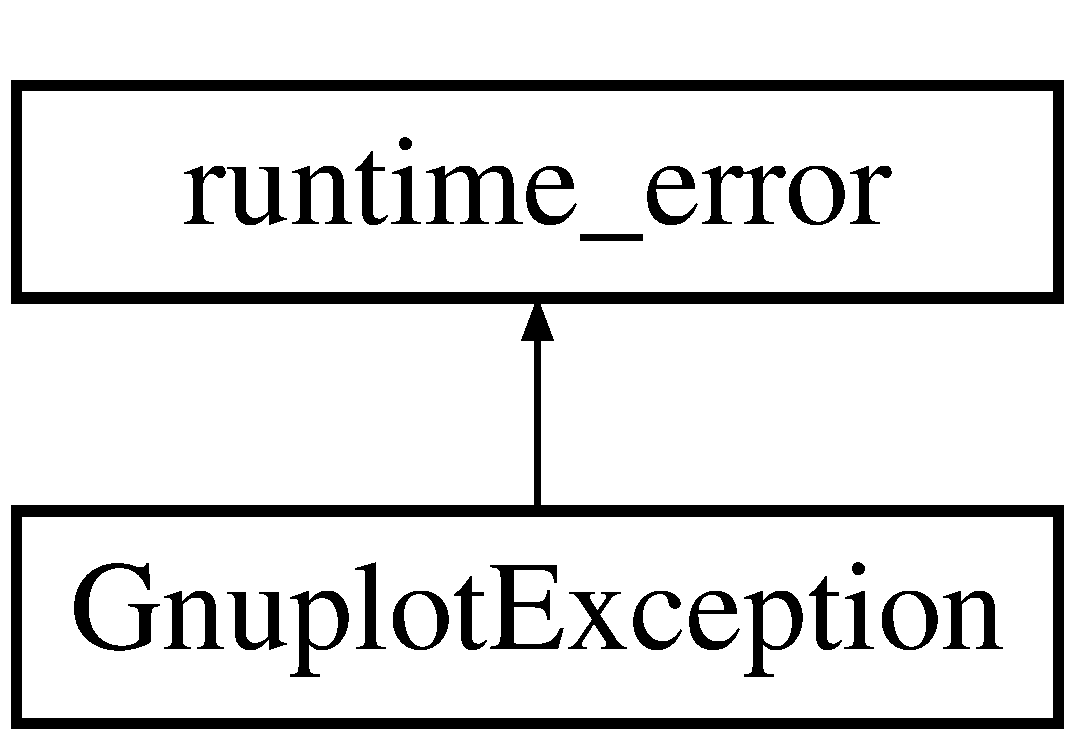
\includegraphics[height=2.000000cm]{classGnuplotException}
\end{center}
\end{figure}
\subsection*{Public Member Functions}
\begin{DoxyCompactItemize}
\item 
\hypertarget{classGnuplotException_a8b324a9ef4d3f75079d41ecd61c62d44}{\hyperlink{classGnuplotException_a8b324a9ef4d3f75079d41ecd61c62d44}{Gnuplot\-Exception} (const std\-::string \&msg)}\label{classGnuplotException_a8b324a9ef4d3f75079d41ecd61c62d44}

\begin{DoxyCompactList}\small\item\em Construtor. \end{DoxyCompactList}\end{DoxyCompactItemize}


\subsection{Detailed Description}
Erros em tempo de execucao. 

The documentation for this class was generated from the following file\-:\begin{DoxyCompactItemize}
\item 
cgnuplot.\-h\end{DoxyCompactItemize}

%--- End generated contents ---

% Index
\newpage
\phantomsection
\addcontentsline{toc}{chapter}{Index}
\printindex

\end{document}
